\begin{exercise}

Die Gleichung

\begin{align*}
  \frac{x^2}{a^2} + \frac{y^2}{b^2} = 1
\end{align*}

beschreibt eine Ellipse in der Ebene.
Zeichnen Sie die Ellipse.
Bestimmen Sie einen Tangentialvektor, einen Normalvektor und die Gleichung der Tangente an die Ellipse in einem beliebigen Punkt $(x_0, y_0)$ der Ellipse.
Machen Sie dies auf zwei Arten:

\begin{enumerate}[label = \textbf{\alph*)}]

  \item durch Auflösen der Gleichung nach $x$ oder $y$.

  \item unter Verwendung der Parametrisierung
  \begin{align*}
    x(t) = a \cos{t},
    \quad
    y(t) = b \sin{t},
    \quad
    t \in [0, 2 \pi].
  \end{align*}

\end{enumerate}

\end{exercise}

\begin{solution}

Die Ellipse $E$ ist also

\begin{align*}
  E :=
  \Bbraces
  {
    (x, y) \in \R^2:
    \frac{x^2}{a^2} + \frac{y^2}{b^2} = 1
  }
\end{align*}

und sieht wie folgt aus.

\begin{figure}[h!]
  \centering
  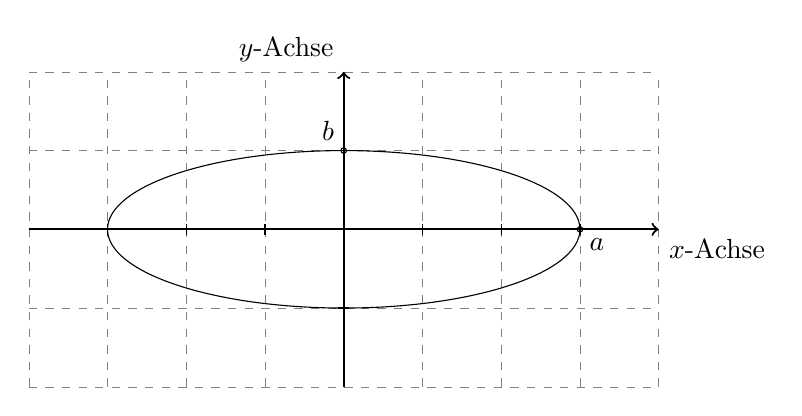
\begin{tikzpicture}

\draw
[step = 1cm, gray, very thin, dashed]
(-4, -2) grid (4, 2);

\draw
[thick, ->]
(-4, 0) -- (4, 0)
node[anchor = north west]{$x$-Achse};

\draw
[thick, ->]
(0, -2) -- (0, 2)
node[anchor = south east]{$y$-Achse};

\foreach \x in {-3, -2, -1, 0, 1, 2, 3}
  \draw (\x cm, 2pt) -- (\x cm, -2pt);

\foreach \y in {-1, 0, 1}
  \draw (2pt, \y cm) -- (-2pt, \y cm);

\draw (0, 0) ellipse (3cm and 1cm);

\draw
(3, 0) circle (1pt)
node[anchor = north west]{$a$};

\draw
(0, 1) circle (1pt)
node[anchor = south east]{$b$};

\end{tikzpicture}

  \caption{Ellipse}
\end{figure}

(a) Wir lösen die Gleichung nach $y$ auf und erhalten

\begin{align*}
  y_\pm = \pm b \sqrt{1 - \pbraces{\frac{x}{a}}^2}.
\end{align*}

Fasst man das als Funktion von $x$ auf so ergibt sich für die Ableitung

\begin{align*}
  y^\prime_{\pm}(x)
  =
  \mp \frac{2bx}{a^2 \sqrt{1 - \pbraces{\frac{x}{a}}^2}}.
\end{align*}

Ein Tangentialvektor $\vec{t}(x_0, y_0)$ im Punkt $(x_0, y_0)^T \in E$ der Ellipse ist

\begin{align*}
  \vec{t}(x_0, y_0)
  =
  \begin{cases}
    (1, y_+^\prime(x_0))^T,
    & \text{wenn} \enspace y_0 > 0, \\
    (0, 1)^T,
    & \text{wenn} \enspace y_0 = 0, \\
    (1, y_-^\prime(x_0))^T,
    & \text{wenn} \enspace y_0 < 0.
  \end{cases}
\end{align*}

Ein Normalvektor $\vec{n}(x_0, y_0)$ im Punkt $(x_0, y_0)^T \in E$ der Ellipse ist

\begin{align*}
  \vec{n}(x_0, y_0)
  =
  \begin{cases}
    (-y_+^\prime(x_0), 1)^T
    & \text{wenn} \enspace y_0 > 0, \\
    (0, 1)^T
    & \text{wenn} \enspace y_0 = 0, \\
    (-y_-^\prime(x_0), 1)^T
    & \text{wenn} \enspace y_0 < 0.
  \end{cases}
\end{align*}

Die Tangentialebene $\vec{T}(x_0, y_0)$ im Punkt $(x_0, y_0)^T \in E$ der Ellipse ist

\begin{align*}
  \vec{T}(x_0, y_0)
  =
  \Bbraces
  {
    (x, y) \in \R^2:
    y =
    \begin{cases}
      y_0 + (x - x_0)y_+^\prime(x_0)
      & \text{wenn} \enspace y_0 > 0 \\
      \pm a
      & \text{wenn} \enspace y_0 = 0 \land x_0 = \pm a \\
      y_0 + (x - x_0) y_-^\prime(x_0)
      & \text{wenn} \enspace y_0 < 0
    \end{cases}
  }.
\end{align*}

(b) Nun parametrisieren wir die Ellipse gemäß Angabe. Ein Tangentialvektor $\vec{t}(t)$ in Abhängigkeit von $t$ ist

\begin{align*}
  \vec{t}(t)
  =
  \begin{pmatrix}
    x^\prime(t) \\ y^\prime(t)
  \end{pmatrix}
  =
  \begin{pmatrix}
    -a \sin(t) \\ b \cos(t)
  \end{pmatrix}.
\end{align*}

Ein Normalvektor $\vec{n}(t)$ in Abhängigkeit von $t$ ist

\begin{align*}
  n(t)
  =
  \begin{pmatrix}
    b \cos(t) \\ a \sin(t)
  \end{pmatrix}.
\end{align*}

Die Tangentialebene $\vec{T}(t)$ in Abhängigkeit von $t$ ist

\begin{align*}
  \vec{T}(t)
  =
  \Bbraces
  {
    (x, y) \in \R^2:
      \begin{cases}
        b \sin(t) - (x - a \cos(t)) \frac{b \cos(t)}{a \sin(t)} = y
        & \text{wenn} \enspace \sin(t) \neq 0 \\
        x = \pm a
        & \text{wenn} \enspace \sin(t) = 0 \land \cos(t) = \pm 1
      \end{cases}
  }.
\end{align*}

Alternativ kann man aus dem Normalvektor die Gleichung für die Tangentialebene ablesen.

\begin{align*}
  b \cos(t) x + a \sin(t) y
  =
  ab \pbraces{\cos^2(t) + \sin^2(t)}
  =
  ab
\end{align*}

\end{solution}
